%% implementation_1_report.tex
%% V1.0
%% 2017/4/11
%% by SR Kanna, Ramcharan Sudarsanam, Preston Wipf
%%*************************************************************************

\documentclass[journal]{IEEEtran}

\usepackage[letterpaper,left=0.75in,right=0.75in,%
  top=1.5in,bottom=0.75in]{geometry}
\usepackage{listings}
\usepackage{color}
\usepackage{hyperref}
\usepackage[english]{babel}
\usepackage{graphicx}
\usepackage{caption}

\definecolor{codegreen}{rgb}{0,0.6,0}
\definecolor{codegray}{rgb}{0.5,0.5,0.5}
\definecolor{codepurple}{rgb}{0.58,0,0.82}
\definecolor{backcolor}{rgb}{0.95,0.95,0.92}

\lstdefinestyle{single}{
  backgroundcolor=\color{backcolor},
  breaklines=false,
  numbers=none,
  keepspaces=false
}

\lstdefinestyle{mystyle}{
  backgroundcolor=\color{backcolor},
  commentstyle=\color{codegreen},
  keywordstyle=\color{magenta},
  numberstyle=\color{codegray},
  stringstyle=\color{codepurple},
  basicstyle=\footnotesize,
  breakatwhitespace=false,
  breaklines=true,
  captionpos=b,
  keepspaces=true,
  numbers=left,
  numbersep=5pt,
  showspaces=true,
  tabsize=2
}

\hyphenation{op-tical net-works semi-conduc-tor}
\lstset{style=mystyle}

\begin{document}
\onecolumn

\title{Implementation 1}
\author{SR~Kanna,~Ramcharan~Sudarsanam,~Preston~Wipf}%

\markboth{Machine Learning and Data Mining, No.~1, April~2017}%
{Shell \MakeLowercase{\textit{et al.}}: Implementation 1}

\maketitle
\bigskip



\section{Problem 1/2}
\noindent [[  3.95843212e+01] \newline
\noindent [ -1.01137046e-01] \newline
\noindent [  4.58935299e-02] \newline
\noindent [ -2.73038670e-03] \newline
\noindent [  3.07201340e+00] \newline
\noindent [ -1.72254072e+01] \newline
\noindent [  3.71125235e+00] \newline
\noindent [  7.15862492e-03] \newline
\noindent [ -1.59900210e+00] \newline
\noindent [  3.73623375e-01] \newline
\noindent [ -1.57564197e-02] \newline
\noindent [ -1.02417703e+00] \newline
\noindent [  9.69321451e-03] \newline
\noindent [ -5.85969273e-01]] \newline
\medskip

\section{Problem 3}
\noindent SSE Training data: 9561.19128998 \newline
\noindent SSE Testing data:  1675.23096595 \newline
\medskip

\section{Problem 4}
\noindent SSE Training data: 9561.19128998 \newline
\noindent SSE Testing data:  1675.23096595 \newline
\noindent The SSE, or loss, increases as when we lose the dummy variable.
Because the dummy variable correlates to our \textit{b} or \textit{w\textsubscript{0}},
which is what translates our line of best fit, removing the variable creates a less
accurate prediction. \newline
\medskip

\section{Problem 5}
\begin{figure}[!h]
\centering
\captionsetup{justification=centering,margin=2cm}
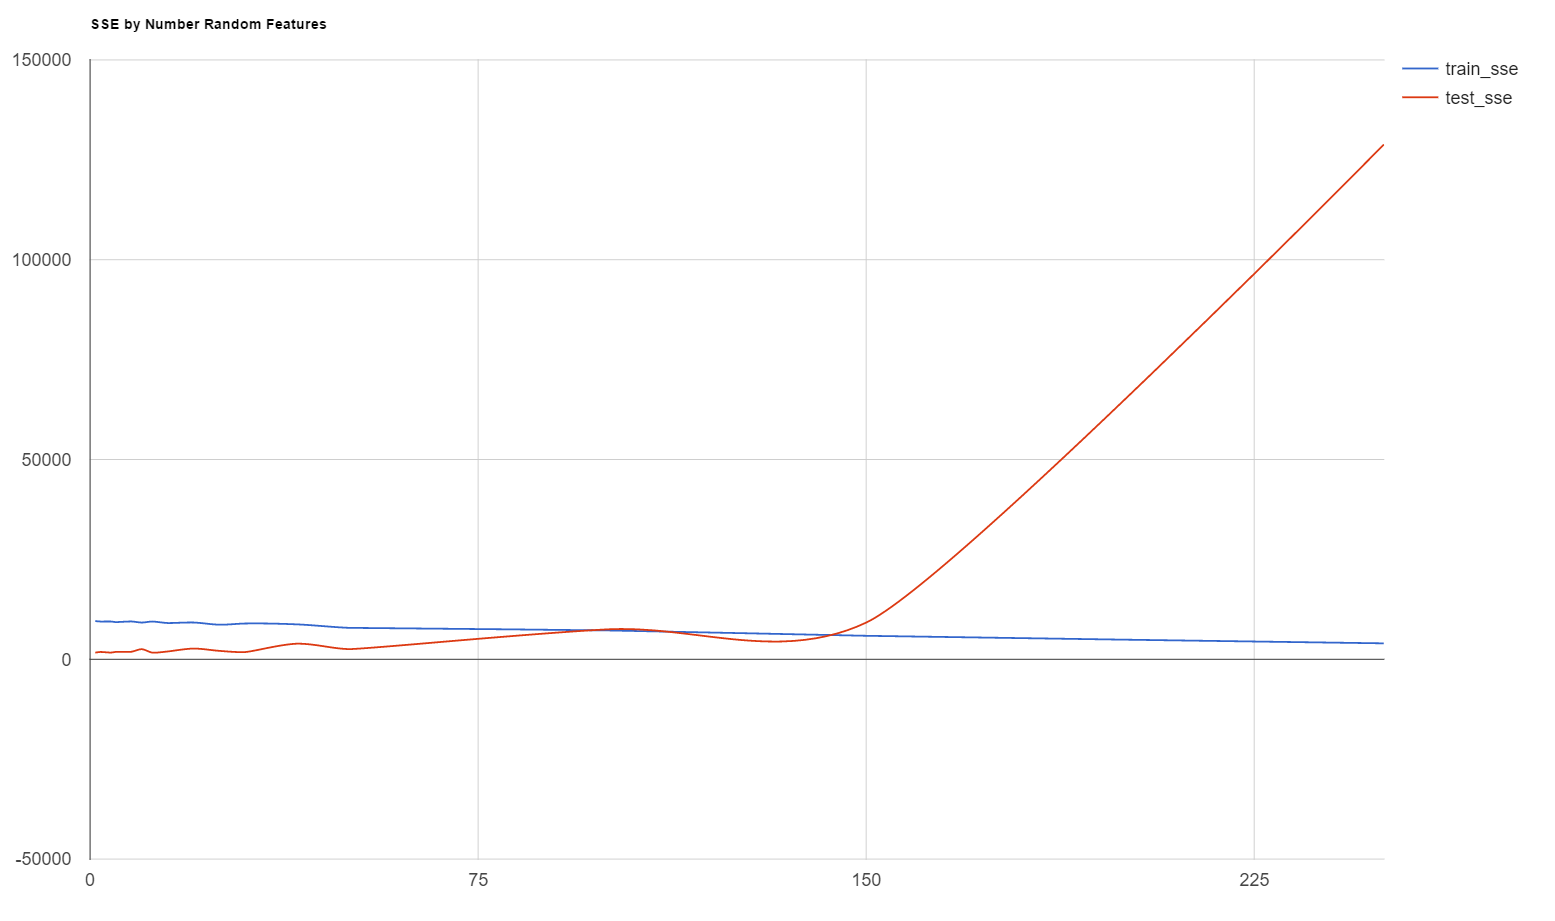
\includegraphics[width=0.9\textwidth]{sse_rand_features.PNG}
\caption{\label{fig:sse}Training SSE decreases linearly; Testing SSE increases exponentially.}
\end{figure}
\smallskip
\noindent Based on the plot above, as more random, uniformly-distributed features
are added to the datasets, the SSE of the training predictions decrease linearly,
but the SSE of the testing data increases exponentially. Intuitively, this is the
result of the model being trained very specifically to match the training dataset,
which creates a better prediction particular to the training dataset due to overfitting
and results in a far worse prediction of the testing dataset. \newline
\medskip

\section{Problem 6}
\begin{figure}[!h]
\centering
\captionsetup{justification=centering,margin=2cm}
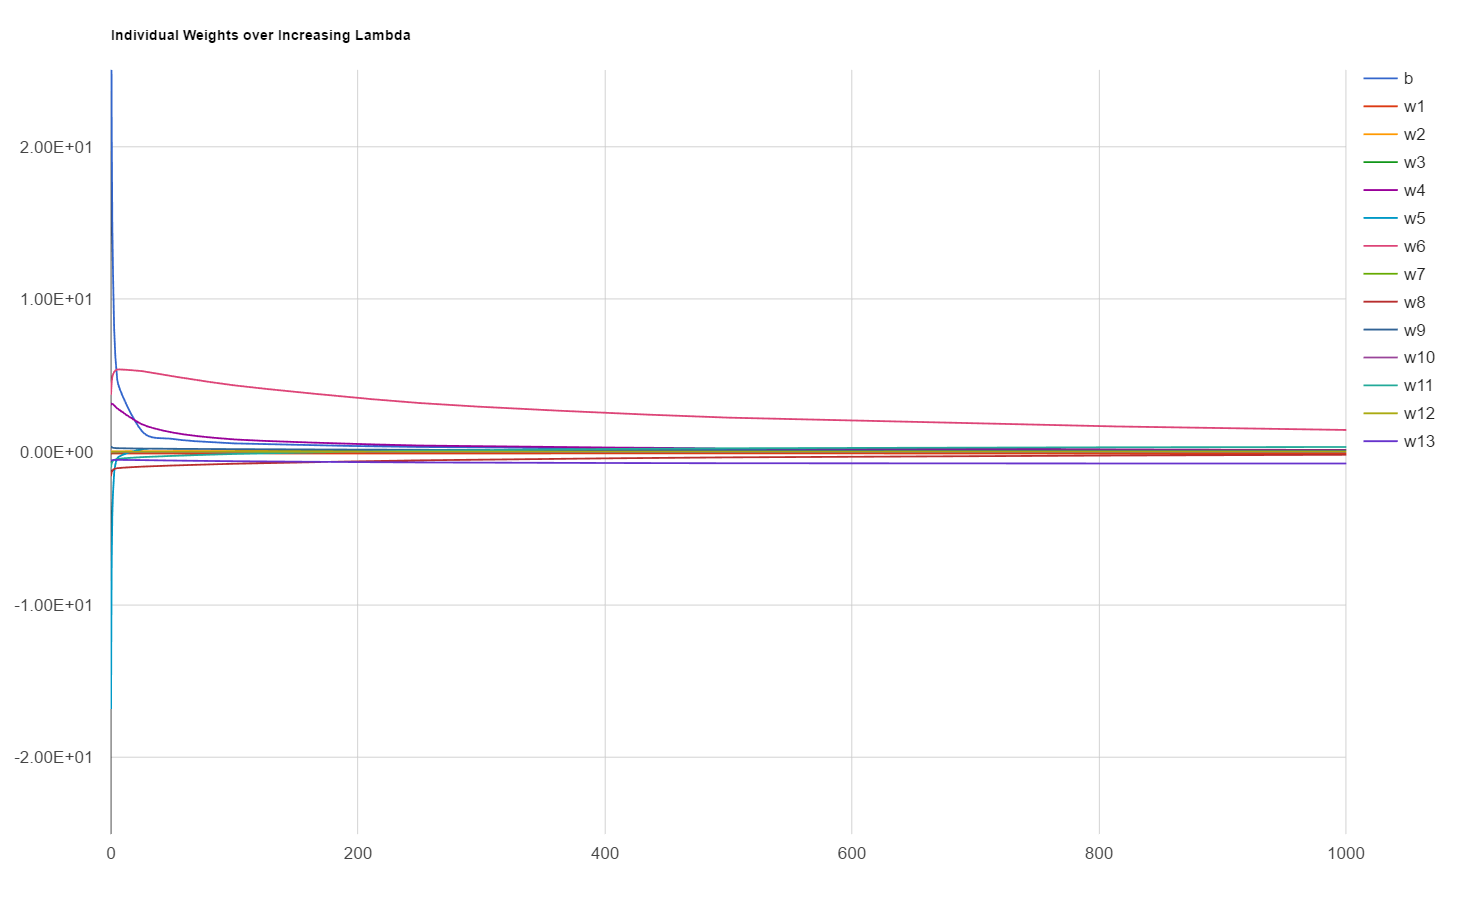
\includegraphics[width=0.9\textwidth]{weights_lambda.PNG}
\caption{\label{fig:lambdas}The weights converge to 0 as the lambda increases.}
\end{figure}
\smallskip
\noindent 
\medskip

\section{Problem 7}
\noindent Looking at the plot, as lambda increases the weights of each feature
begin to converge to 0. Given a large enough lambda, the weights are essentially
0, meaning each weight holds nearly no predictive power. \newline
\medskip

\section{Problem 8}
\noindent Based on this equation, we sum across two terms: the standard SSE
and the regularization term. As values of lambda increase, the regularization
term dominates the summation. As lambda decreases, the SSE term dominates the
summation. The summation as a whole represents the loss of the model; if we
are therefore minimizing loss, for large values of lambda we will prioritize
small magnitudes of \textit{w}. On the other hand, for small values of lambda,
we are prioritizing the closest fit possible. \\

\noindent Looking at our chart then, it makes sense that as we increase the
value of lambda the calculated weights are made forcibly smaller to accomodate
our increasing prioritization of regularization. \newline
\medskip

 

\end{document}
